\section{Monitors}
\label{sec:method}

Let a clip be a frame sequence $f_0,\dots,f_{T-1}$ with $T=30$. Every monitor
emits one scalar per frame and must be a function of $f_{\leq t}$ alone. We
enforce this structurally: each monitor is a streaming object that receives one
latent at a time and holds no forward state, so referencing a future frame is
not something the implementation can express. Section~\ref{sec:protocol}
describes the adversarial test that confirms it.

\subsection{Latent state}

V-JEPA 2 embeds video with a $3$D convolution of stride
$(\tau, p, p)$ for tubelet size $\tau=2$ and patch size $p=16$, followed by a
flatten-and-transpose. The token sequence is therefore \emph{t-major}: token $i$
belongs to tubelet $\lfloor i / (H'W') \rfloor$, where $H'W'$ is the number of
spatial patches. Tubelet $j$ owns the contiguous index block
$[\,jH'W',\,(j{+}1)H'W'\,)$. Every index computation below rests on this, and we
verify it directly against the patch embedder rather than assuming it.

Because the tubelet spans two frames, no V-JEPA 2 representation is a function
of a single frame; the protocol's notion of a ``per-frame latent'' has to be
made precise. Define the \textbf{causal window} ending at $t$,
\begin{equation}
W_t \;=\; \bigl(f_{\max(t-T_{\mathrm{ctx}}+1,\,0)},\,\dots,\,f_t\bigr),
\qquad T_{\mathrm{ctx}} = 16,
\end{equation}
left-padded by repeating $f_0$. Let $E(\cdot)$ be the frozen encoder and
$E_j(\cdot)$ its output tokens for tubelet $j$. With
$J = T_{\mathrm{ctx}}/\tau - 1$ the final tubelet index, the latent state is the
spatial mean of the final tubelet,
\begin{equation}
z_t \;=\; \frac{1}{H'W'} \sum_{k} \bigl[E_J(W_t)\bigr]_k \;\in\; \mathbb{R}^{d},
\qquad d = 1024 .
\end{equation}
The final tubelet spans frames $(t{-}1, t)$, so $z_t$ depends on no frame later
than $t$. All three probes are functions of the sequence $\{z_t\}$ alone.

\subsection{Baseline \texorpdfstring{$\mathcal{L}_0$}{L0}: the model's own loss,
evaluated causally}

V-JEPA 2's pretraining objective predicts the representation of masked target
tokens from context tokens. Evaluating it online requires care. The reference
implementation runs \emph{one} encoder pass over the full video and then applies
masks, so the context tokens have attended to the frames being predicted; its
own source notes that training instead uses a separate target encoder. Using
that single-pass loss as our baseline would let the context see the answer,
inflating the baseline and biasing against the hypothesis.

We therefore use two encoder passes. Define the \textbf{context window}
\begin{equation}
W'_t \;=\; \bigl(f_{t-15},\,\dots,\,f_{t-2},\,f_{t-2},\,f_{t-2}\bigr),
\end{equation}
that is, $W_t$ with its final tubelet overwritten by a repeat of $f_{t-2}$.
Tubelets $0..J{-}1$ of $W'_t$ are exactly frames $f_{t-15..t-2}$, and no token
in them can attend to $f_{t-1}$ or $f_t$ (Figure~\ref{fig:windows}). Writing
$P(\cdot \mid \cdot)$ for the frozen predictor applied to those context tokens
with the final tubelet's positions as targets,
\begin{equation}
\mathcal{L}_0(t) \;=\;
\bigl\lVert\, P\bigl(E_{0:J-1}(W'_t)\bigr) \;-\; E_J(W_t) \,\bigr\rVert_2^2 \big/ (H'W'd),
\end{equation}
the mean squared error between the prediction and the true final-tubelet
tokens. The target is allowed to depend on $f_t$ --- it \emph{is} the quantity
revealed at time $t$ --- while the prediction is not.

\begin{figure}[t]
\centering
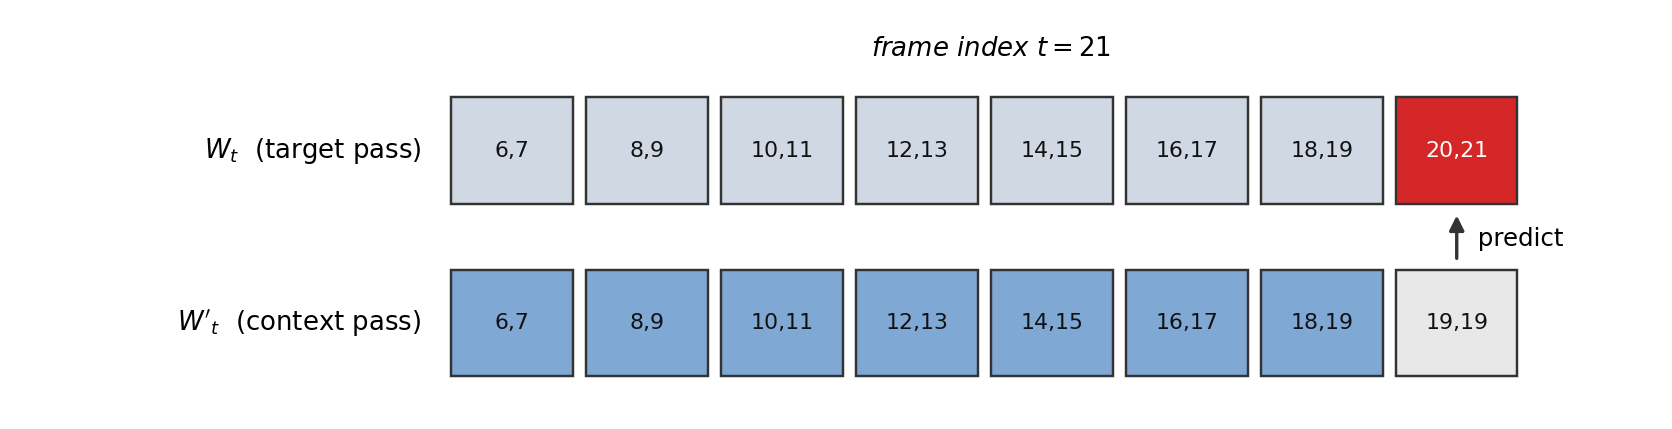
\includegraphics[width=\linewidth]{generated/fig_windows.png}
\caption{The two encoder passes used at frame $t$. Each box is one $2$-frame
tubelet, labelled by the frames it spans. The context pass $W'_t$ overwrites the
final tubelet with a repeat of $f_{t-2}$, so the predictor's context is a
function of $f_{\leq t-2}$ only, while the target comes from the full window
$W_t$. A single-pass implementation would let the context attend to
$f_{t-1},f_t$ and make the loss partly self-fulfilling.}
\label{fig:windows}
\end{figure}

\subsection{Baseline \texorpdfstring{$\mathcal{L}_1$}{L1}: information-matched
prediction error}

$\mathcal{L}_0$ and the geometry probes consume different representations ---
token grids versus a pooled vector --- which invites the objection that any
difference between them is an artefact of what they see. We therefore add a
second baseline that consumes \emph{exactly} the sequence the probes do. Let
$W^\star$ be a ridge map fitted to predict $z_t$ from its two predecessors,
\begin{equation}
W^\star = \arg\min_{W} \sum \bigl\lVert z_t - W[z_{t-1}; z_{t-2}] \bigr\rVert_2^2
+ \lambda \lVert W \rVert_F^2 , \qquad \lambda = 1,
\end{equation}
fitted on control-calibration clips only, and
$\mathcal{L}_1(t) = \lVert z_t - W^\star[z_{t-1};z_{t-2}] \rVert_2$. Scores for
the calibration clips themselves are produced by $5$-fold cross-fitting, so
$\mathcal{L}_1$'s own threshold is not optimistic. A probe must beat
\emph{both} baselines to count.

\subsection{Geometry probes}

All three are computed online from $\{z_t\}$ with no normalisation.

\begin{align}
\text{A. Trajectory curvature:}\quad
  a_t &= \bigl\lVert z_t - 2 z_{t-1} + z_{t-2} \bigr\rVert_2
  \label{eq:probeA}\\[2pt]
\text{B. Representational distance:}\quad
  b_t &= 1 - \frac{\langle z_t,\ \bar z_t \rangle}{\lVert z_t\rVert\,\lVert \bar z_t\rVert},
  \qquad \bar z_t = \tfrac{1}{5}\textstyle\sum_{i=1}^{5} z_{t-i}
  \label{eq:probeB}\\[2pt]
\text{C. Covariance shift:}\quad
  c_t &= \bigl\lVert \Sigma_t - \Sigma_{\mathrm{base}} \bigr\rVert_F,
  \qquad \Sigma_t = \widehat{\mathrm{Cov}}(z_{t-4..t})
  \label{eq:probeC}
\end{align}
where $\Sigma_{\mathrm{base}} = \widehat{\mathrm{Cov}}(z_{0..14})$ is frozen at
$t=14$, and both covariances use $\mathrm{ddof}=1$. Probe~A is a second
difference, probe~B is scale-invariant, probe~C compares second-order structure
against the clip's own pre-injection baseline.

\paragraph{Computing probe C without forming $d \times d$ matrices.}
Written naively, \eqref{eq:probeC} builds two $1024\times1024$ covariances per
frame. Both are low-rank: with centred factors $A \in \mathbb{R}^{k_a \times d}$
and $B \in \mathbb{R}^{k_b \times d}$ and $\Sigma = A^\top A/(k{-}1)$, the trace
identities give
\begin{equation}
\lVert \Sigma_a - \Sigma_b \rVert_F^2 =
\frac{\lVert AA^\top \rVert_F^2}{(k_a{-}1)^2}
- \frac{2\,\lVert AB^\top \rVert_F^2}{(k_a{-}1)(k_b{-}1)}
+ \frac{\lVert BB^\top \rVert_F^2}{(k_b{-}1)^2},
\end{equation}
which costs $O(k^2 d)$ instead of $O(d^2 k)$ and touches only $k \times k$
Grams. We verify it against the naive computation to machine precision
($\leq 2\times10^{-16}$ relative).

\paragraph{A numerical caveat.}
Probe~A is a second difference of nearby vectors, the textbook setting for
catastrophic cancellation: relative error in $z$ is amplified. Reduced-precision
inference is therefore not a free speed-up here, and we measure fp32 against
bf16 and fp16 on the actual probe values rather than assuming a choice is safe.
